\documentclass{ximera}
\usepackage{sagetex}
%% handout
%% space
%% newpage
%% numbers
%% nooutcomes

%% You can put user macros here
%% However, you cannot make new environments

\graphicspath{{./}{module1Activity/}{module2Activity/}{module3Activity/}}

\usepackage{sagetex}
\usepackage{tikz}
\usepackage{hyperref}
\usepackage{tkz-euclide}
\usetkzobj{all}
\pgfplotsset{compat=1.7} % prevents compile error.

\tikzstyle geometryDiagrams=[ultra thick,color=blue!50!black]
 %% we can turn off input when making a master document

\outcome{Recognize and construct linear functions as well as solve linear equations.}
\author{Darryl Chamberlain Jr.}
 
\title{Objective 3 - Convert between a linear equation and its graph.}

\begin{document}
\begin{abstract}
Constructing the linear equation based on its graph. 
\end{abstract}
\maketitle

\href{https://cnx.org/contents/mwjClAV_@8.1:62_eXnY6@14/Linear-Equations-in-One-Variable}{Link to section in online textbook.}

%%%%%%%%%%%%%%%%%%%%%
%%%  Objective 1  %%%
%%%%%%%%%%%%%%%%%%%%%

First, watch \underline{\href{https://mediasite.video.ufl.edu/Mediasite/Play/be61784320d14422820fb6f774fd7b7b1d}{this video}} to learn how to convert from a graph to its linear function. 


\begin{question}
Write the equation of the line in the graph below in Slope-Intercept form and in Standard form. 

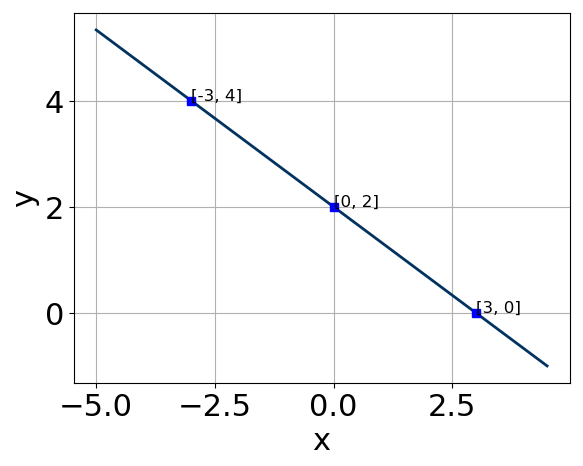
\includegraphics[scale=0.5]{question1.png}

Slope-Intercept form: $y = \answer{-2/3}x + \answer{2}$

Standard form: $\answer{2} x + \answer{3} y = \answer{6}$

\begin{hint}
	What do we know about the coefficients in Standard Form? Is there anything special about the coefficient for $x$?
\end{hint}
\end{question}

\begin{question}
Write the equation of the line in the graph below in Slope-Intercept form and in Standard form. 

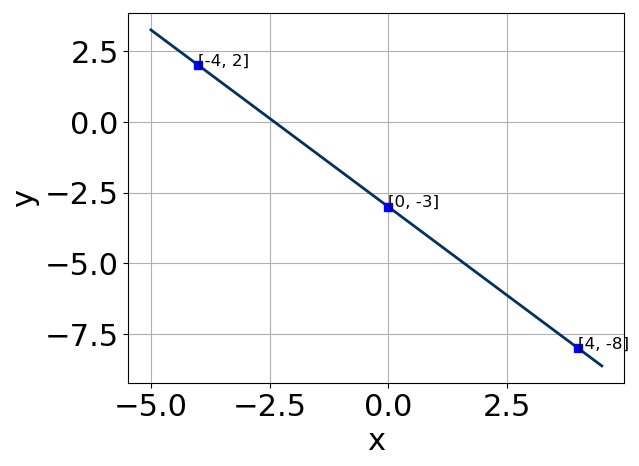
\includegraphics[scale=0.5]{question2.png}

Slope-Intercept form: $y = \answer{-5/4}x + \answer{-3}$

Standard form: $\answer{5} x + \answer{4} y = \answer{-12}$

\begin{hint}
	What do we know about the coefficients in Standard Form? Is there anything special about the coefficient for $x$?
\end{hint}
\end{question}

\begin{question}
Write the equation of the line in the graph below in Slope-Intercept form and in Standard form. 

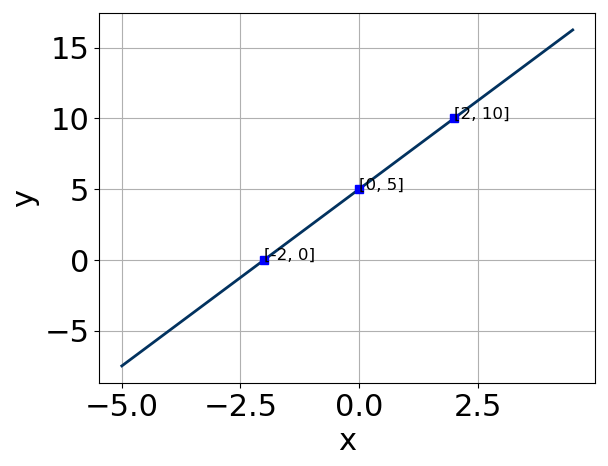
\includegraphics[scale=0.5]{question3.png}

Slope-Intercept form: $y = \answer{5/2}x + \answer{5}$

Standard form: $\answer{5} x + \answer{-2} y = \answer{-10}$

\begin{hint}
	What do we know about the coefficients in Standard Form? Is there anything special about the coefficient for $x$?
\end{hint}
\end{question}

\end{document}